\chapter{Architectural Views} \label{ArchitecturalViews}

\section{Context View}

The context view provides an overview of the FarmBot system, illustrating how it interacts with external entities. It includes the system's scope, boundaries, and its relationships with other systems and stakeholders. The primary purpose of this view is to present a high-level understanding of the system's environment and its external dependencies.
\subsection{Stakeholders’ Uses of This View}

The context view is utilized by various stakeholders to understand the high-level interactions and dependencies of the FarmBot system. Key stakeholders and their uses of this view include:

\begin{itemize}
    \item \textbf{Developers:} Utilize this view to comprehend the system's external interfaces and dependencies, which aids in integrating new features and troubleshooting issues.
    \item \textbf{System Architects:} Use the context view to ensure that the system's design aligns with its environmental constraints and interactions with external entities.
    \item \textbf{Project Managers:} Reference this view to understand the scope of the system, helping in resource allocation and project planning.
    \item \textbf{End Users:} Gain insights into how the system interacts with external services like weather data providers and cloud services, ensuring transparency and trust in the system's operations.
    \item \textbf{Educators:} Leverage this view to explain the system's architecture and its interactions with external entities to students, promoting an understanding of precision agriculture technologies.
    \item \textbf{Maintenance Teams:} Use the context view to identify potential external factors that may affect system performance and to plan for maintenance activities accordingly.
\end{itemize}

This high-level perspective helps stakeholders ensure that FarmBot operates efficiently within its intended environment and meets the needs of its users.

\subsubsection{External Entities}
\begin{itemize}
    \item \textbf{Users:} Gardeners, small-scale farmers, and educators who interact with the FarmBot system via the web-based and mobile applications.
    \item \textbf{Weather Data Providers:} External services that supply weather forecasts and real-time weather data to optimize FarmBot's operations.
    \item \textbf{Agricultural Databases:} Sources of information on plant species, soil types, and pest control, used by FarmBot to make informed decisions.
    \item \textbf{Sensor Systems:} Hardware components that provide real-time data on soil moisture, temperature, and other environmental factors.
    \item \textbf{Cloud Services:} Platforms for data storage, processing, and remote access to FarmBot's operational logs and user preferences.
\end{itemize}

\subsubsection{System Boundaries}
FarmBot is an autonomous precision agriculture system designed to operate within the boundaries of a small-scale garden or farm. It consists of hardware components like the Farmduino electronics board, soil moisture sensors, and the Raspberry Pi, along with a software platform that includes scheduling, monitoring, and control functionalities.




\subsection{Context Diagram}
The context diagram for the FarmBot system provides a visual representation of the system's external interfaces and interactions with various external entities. This diagram is critical for understanding how FarmBot integrates with its environment and other systems.

This context diagram illustrates the interconnected nature of FarmBot's components 
\begin{figure}[H]
    \centering
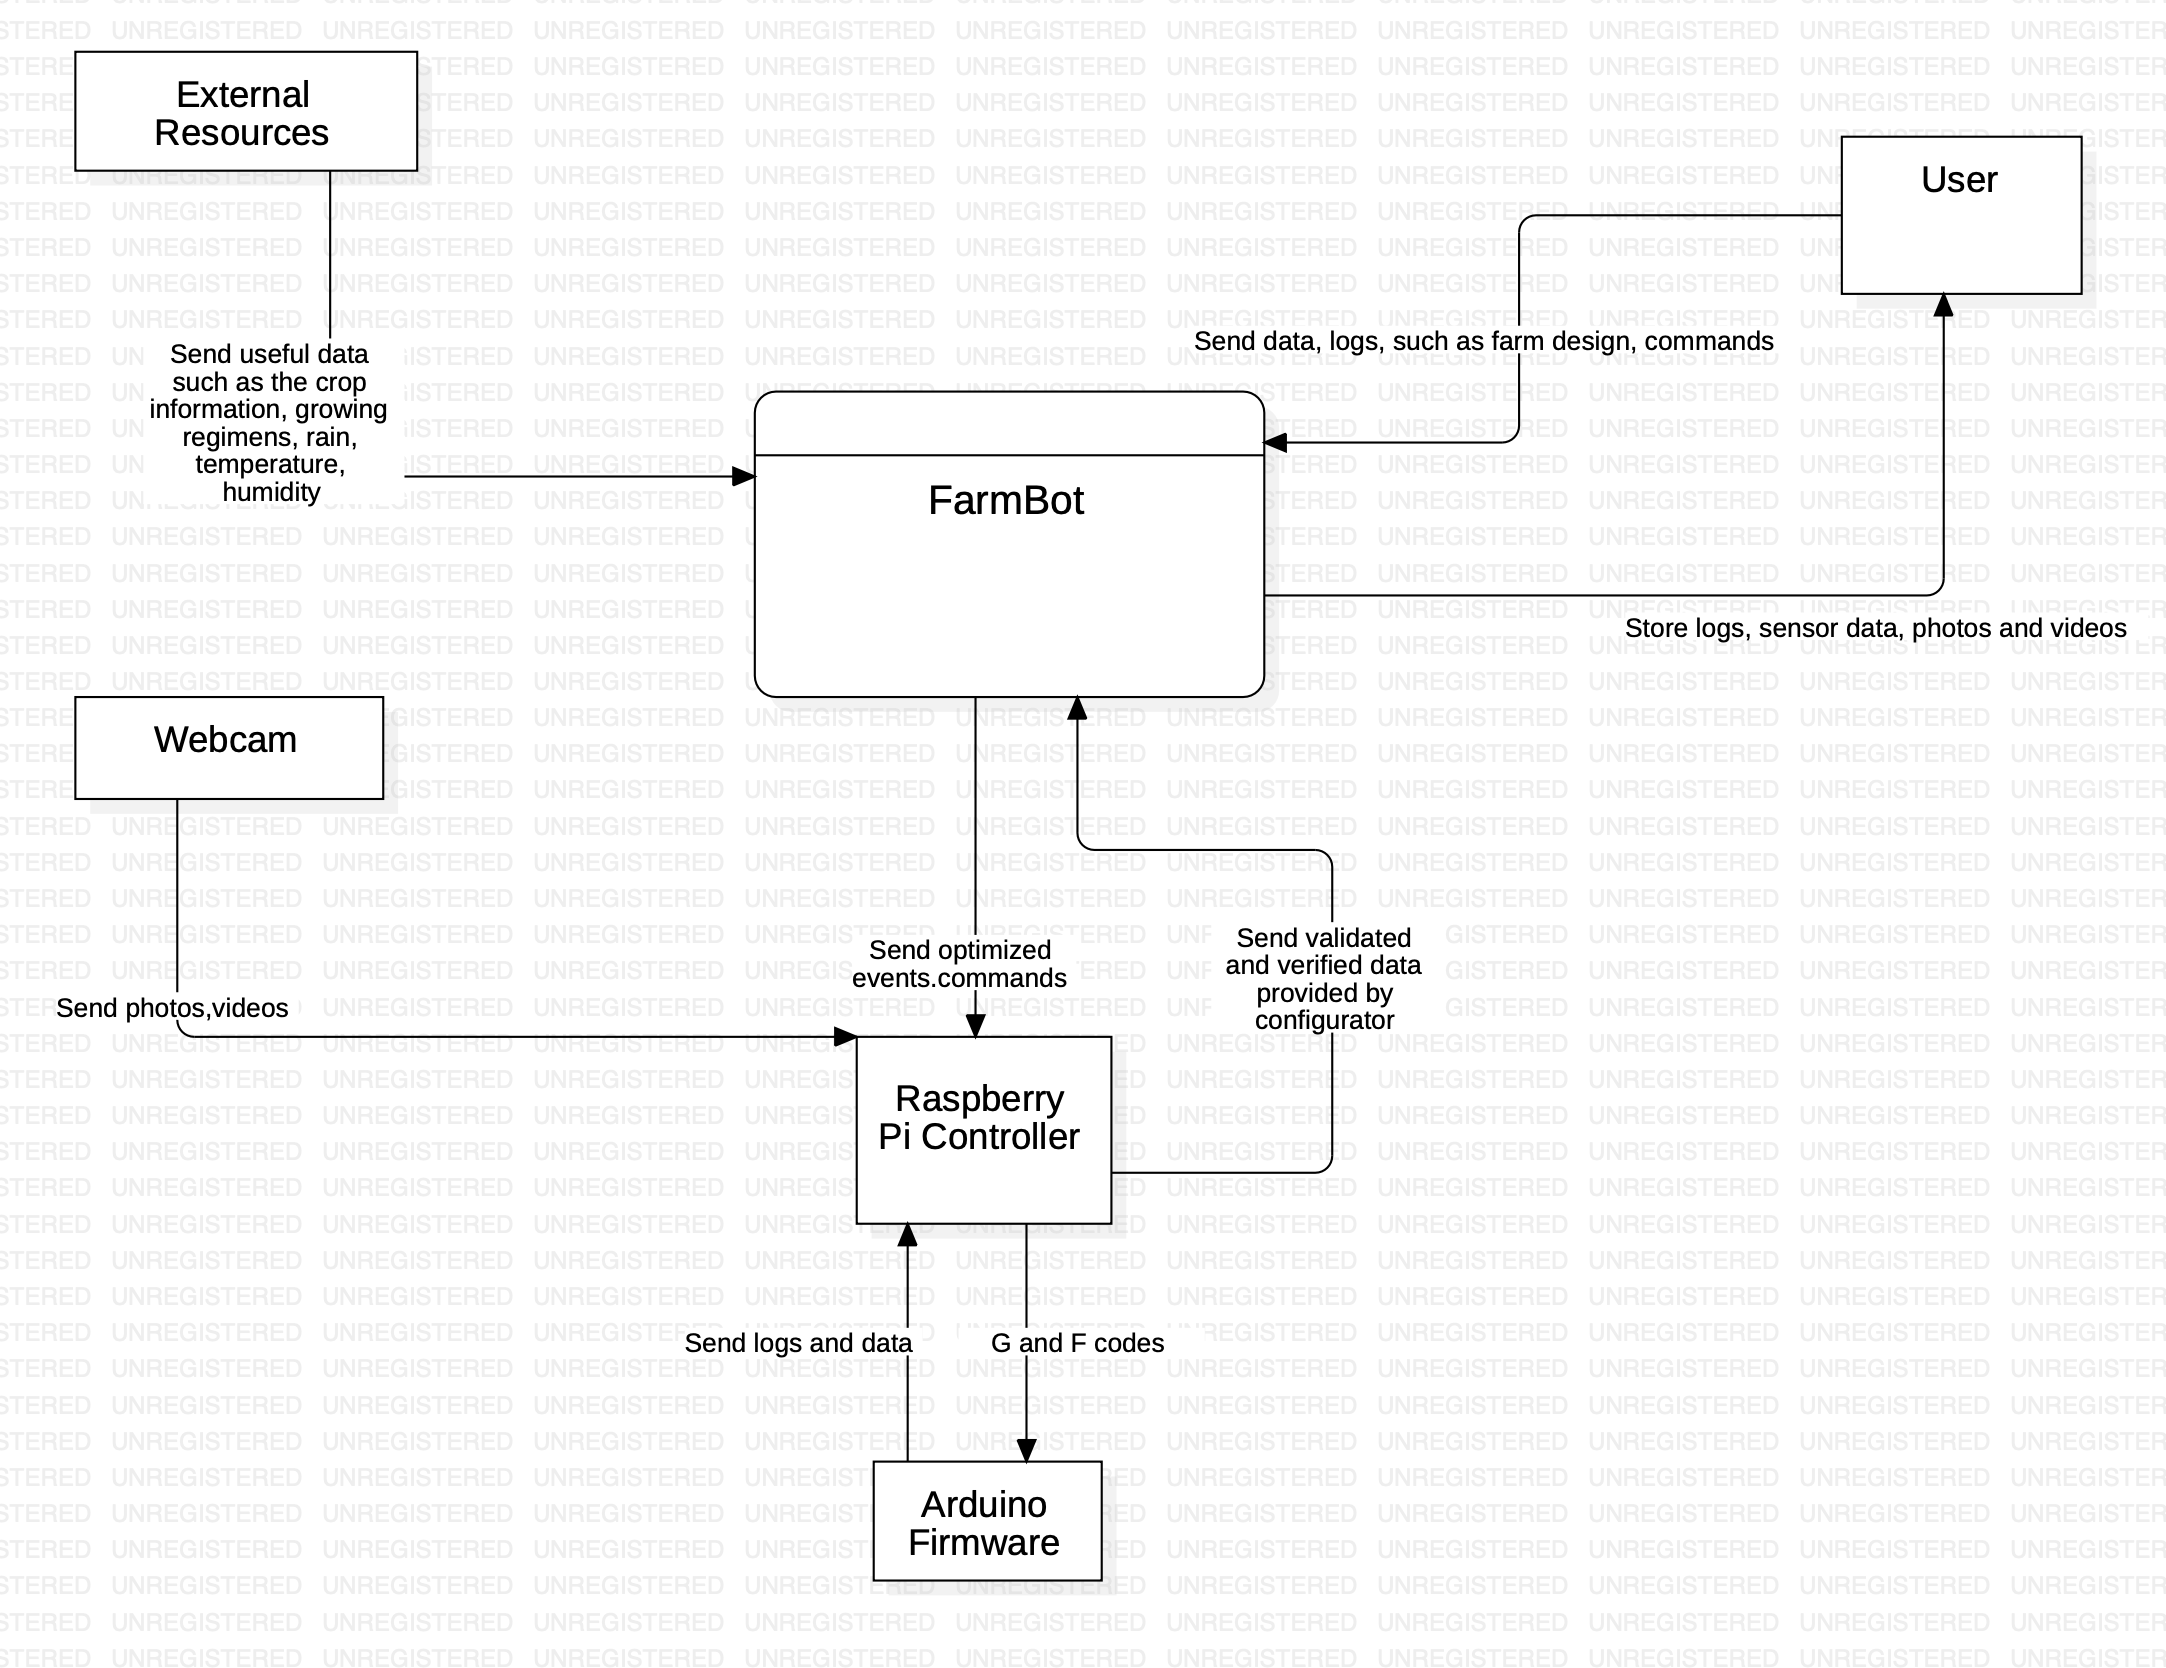
\includegraphics[scale=0.2]{./Figures/farmbot_context_diagram.png}
\caption{FarmBot Context Diagram}
\end{figure}

\subsubsection{FarmBot}
At the center of the diagram is FarmBot itself, which acts as the core operational system. FarmBot is responsible for executing all automated farming tasks such as planting, watering, and weeding, based on inputs it receives from the user and external resources.

\subsubsection{External Resources}
\textbf{Description:} External Resources represent various data sources that FarmBot utilizes to make informed decisions and optimize its operations. These include:
\begin{itemize}
    \item \textbf{Weather Data:} Information such as temperature, rainfall, and humidity, which are crucial for planning and adjusting farming activities.
    \item \textbf{Soil Data:} Data on soil quality and type, helping to customize nutrient application and watering schedules.
\end{itemize}

\subsubsection{User}
\textbf{Description:} The user interacts with FarmBot via a dedicated interface that allows for monitoring and manual control when necessary. The user's role includes:
\begin{itemize}
    \item \textbf{Sending Commands:} Users can send specific commands to FarmBot for immediate actions or schedule tasks.
    \item \textbf{Receiving Data:} Users receive updates and reports on FarmBot's activities and the status of the garden or farm.
\end{itemize}

\subsubsection{Raspberry Pi Controller}
\textbf{Description:} The Raspberry Pi acts as the central processing unit of FarmBot, controlling its operations and communicating with both the hardware components and the user interface.
\begin{itemize}
    \item \textbf{Data Logging:} It logs detailed operational data including system performance and task logs.
    \item \textbf{Command Execution:} Receives and executes commands from the user interface.
\end{itemize}

\subsubsection{Arduino Firmware}
\textbf{Description:} The Arduino controls the hardware aspects of FarmBot, interfacing directly with the physical components like motors, sensors, and water systems.
\begin{itemize}
    \item \textbf{Direct Hardware Control:} Executes low-level commands sent by the Raspberry Pi to perform physical operations.
    \item \textbf{Sensor Data Collection:} Gathers data from various sensors embedded in the farming environment and sends it to the Raspberry Pi for processing.
\end{itemize}

\subsubsection{Webcam}
\textbf{Description:} The webcam serves as an imaging tool that provides visual feedback to the user and helps in monitoring plant health and growth.
\begin{itemize}
    \item \textbf{Visual Monitoring:} Sends real-time images and videos to the user, allowing for remote monitoring of the farm's condition.
\end{itemize}


\subsection{External Interfaces}
\begin{figure}[H]
    \centering
\includesvg[inkscapelatex=false, scale=0.56]{./Figures/external_interface_class_diagram.svg}
\caption{Class Diagram for External Interfaces}
\end{figure}

The FarmBot system is designed with multiple external interfaces to interact with system elements and external entities, including user input mechanisms and automated data retrieval systems. These interfaces are crucial for the operation of the FarmBot and define how it communicates with the external world.

\subsubsection{User Interface API}
\begin{itemize}
    \item \textbf{Name:} User Interface \gls{api}
    \item \textbf{Purpose:} To allow users to interact with the FarmBot system for monitoring and control purposes.
    \item \textbf{Source of Input:} User through web or mobile interface.
    \item \textbf{Destination of Output:} FarmBot hardware and software systems for execution of tasks.
\end{itemize}


\subsubsection{Sensor Data Interface}
\begin{itemize}
    \item \textbf{Name:} Sensor Data Interface
    \item \textbf{Purpose:} To collect environmental data such as soil moisture and temperature for the FarmBot to make informed decisions.
    \item \textbf{Source of Input:} Environmental sensors deployed within the FarmBot operational area.
    \item \textbf{Destination of Output:} FarmBot's decision support system and user interface for real-time environmental data display.
\end{itemize}

\subsubsection{Remote Update API}
\begin{itemize}
    \item \textbf{Name:} Remote Update API
    \item \textbf{Purpose:} To manage and deploy software updates to the FarmBot system.
    \item \textbf{Source of Input:} Remote update server.
    \item \textbf{Destination of Output:} FarmBot's internal systems to apply updates.
\end{itemize}


\subsubsection{Farming Schedule API}
\begin{itemize}
    \item \textbf{Name:} Farming Schedule API
    \item \textbf{Purpose:} To handle the timing and execution of farming tasks.
    \item \textbf{Source of Input:} User-defined schedules and automated system recommendations.
    \item \textbf{Destination of Output:} FarmBot's actuators and task management system.
\end{itemize}

These interfaces incorporate bi-directional flows of information where applicable, facilitating a responsive and adaptable system. The inputs and outputs defined here are based on the actual FarmBot API documentation for accuracy.

\subsection{Interaction scenarios}

This section includes two activity diagrams to illustrate interaction sequences that take place over the external interfaces. The chosen scenarios represent some of the most complex interactions within the FarmBot system. These diagrams provide a detailed view of how different components and external systems interact to achieve specific functionalities.

\begin{figure}[H]
    \centering
    \includesvg[inkscapelatex=false, scale=0.7]{./Figures/external_interface_sensor_diagram.svg}
    \caption{External Interface Sensor Activity Diagram}
\end{figure}

\subsubsection{External Interface Sensor Interaction}

The first activity diagram illustrates the interaction between the FarmBot system and the external sensor interface. This interaction is critical for gathering real-time environmental data, which is essential for making informed decisions about watering, planting, and other agricultural tasks.

\textbf{Steps in the Interaction Sequence:}
\begin{enumerate}
    \item \textbf{Initialization:} The FarmBot system initializes the sensor interface to start the data collection process.
    \item \textbf{Data Request:} A request for sensor data is sent from the FarmBot controller to the external sensors.
    \item \textbf{Data Collection:} The sensors collect data on various environmental parameters such as soil moisture, temperature, and light intensity.
    \item \textbf{Data Transmission:} The collected data is transmitted back to the FarmBot controller.
    \item \textbf{Data Processing:} The FarmBot system processes the received data to assess the current environmental conditions.
    \item \textbf{Decision Making:} Based on the processed data, the system makes decisions regarding necessary actions, such as adjusting watering schedules or initiating plant health monitoring.
    \item \textbf{Action Execution:} The FarmBot executes the decided actions, ensuring optimal conditions for plant growth.
    \item \textbf{Logging:} All actions and data points are logged for future reference and analysis.
\end{enumerate}

This interaction scenario demonstrates the complexity and importance of seamless communication between FarmBot and its external sensor interfaces, highlighting the system's ability to adapt to real-time environmental changes.

\begin{figure}[H]
    \centering
    \includesvg[inkscapelatex=false, scale=0.7]{./Figures/external_interface_user_diagram.svg}
    \caption{External Interface User Interface Activity Diagram}
\end{figure}

\subsubsection{External Interface User Interface Interaction}

The second activity diagram depicts the interaction between the FarmBot system and the external user interface. This interaction is crucial for obtaining accurate weather forecasts, which help in planning and optimizing various agricultural tasks.

\textbf{Steps in the Interaction Sequence:}
\begin{enumerate}
    \item \textbf{API Initialization:} The FarmBot system initializes a connection to the weather API service.
    \item \textbf{Forecast Request:} A request for weather forecast data is sent from the FarmBot system to the weather API.
    \item \textbf{Data Retrieval:} The weather API processes the request and retrieves the relevant weather forecast data.
    \item \textbf{Data Transmission:} The forecast data is transmitted back to the FarmBot system.
    \item \textbf{Data Analysis:} The FarmBot system analyzes the received weather data to determine potential impacts on agricultural activities.
    \item \textbf{Schedule Adjustment:} Based on the analysis, the system adjusts the scheduling of tasks such as watering, planting, and harvesting to align with the forecasted weather conditions.
    \item \textbf{Notification:} The system sends notifications to the user about the adjusted schedules and any significant weather events that may affect the farm.
    \item \textbf{Logging:} All interactions and adjustments are logged for future analysis and reporting.
\end{enumerate}

This scenario highlights the integration of external weather data into the FarmBot system, showcasing the ability to proactively adjust operations based on forecasted weather conditions.

These interaction scenarios provide a comprehensive view of how the FarmBot system communicates with external interfaces, ensuring efficient and effective agricultural management.

\section{Functional View}

The Functional View provides a detailed perspective on the functionalities of the FarmBot system, illustrating how various components interact to achieve the system's goals. This view is crucial for understanding the operational aspects of the system and how it meets the needs of its users.

\subsection{Stakeholders’ Uses of This View}

The Functional View is utilized by various stakeholders to comprehend the operational workflows and interactions within the FarmBot system. Key stakeholders and their uses of this view include:

\begin{itemize}
    \item \textbf{Developers:} Use this view to understand the interactions between components and to implement or modify system functionalities accordingly.
    \item \textbf{System Architects:} Leverage this view to ensure that the system’s design supports the required functionalities and interactions.
    \item \textbf{Project Managers:} Reference this view to plan and manage development tasks, ensuring that all functional requirements are met.
    \item \textbf{End Users:} Gain insights into how the system's functionalities are structured and how different components work together to provide the desired outcomes.
    \item \textbf{Quality Assurance Teams:} Use this view to design test cases that validate the functional interactions between system components.
    \item \textbf{Maintenance Teams:} Reference this view to understand the functional dependencies and to diagnose and troubleshoot issues effectively.
\end{itemize}

\subsection{Component Diagram}

This section includes a Component Diagram and its explanations for the FarmBot system. The diagram illustrates the core components and their provides/requires relationships.

\begin{figure}[H]
    \centering
    \includesvg[inkscapelatex=false, scale=0.45]{./Figures/farmbot_component_diagram.svg}
    \caption{FarmBot Component Diagram}
\end{figure}

The component diagram includes the following components and their relationships:

\textbf{Core Components:}
\begin{itemize}
    \item \textbf{Web Application:}
    \begin{itemize}
        \item Requires services from the User Management API and Data Processing Module.
    \end{itemize}

    \item \textbf{Main Controller:}
    \begin{itemize}
        \item Provides control over the Sensor Controller, Actuator Controller, Logging Module, and Diagnostics Module.
    \end{itemize}

    \item \textbf{Sensor Controller:}
    \begin{itemize}
        \item Requires data from the Sensor API and Sensors.
        \item Provides data to the Data Processing Module.
    \end{itemize}

    \item \textbf{Actuator Controller:}
    \begin{itemize}
        \item Requires data from the Data Processing Module.
        \item Provides commands to the Actuators.
    \end{itemize}

    \item \textbf{Data Processing Module:}
    \begin{itemize}
        \item Requires data from the Database and Weather API.
        \item Provides processed data to the Main Controller.
    \end{itemize}

    \item \textbf{Network Communication Module:}
    \begin{itemize}
        \item Requires services from the Web Application and Mobile Application.
    \end{itemize}
\end{itemize}

\textbf{Explanations of the Core Components:}

\begin{itemize}
    \item \textbf{Web Application:} Allows users to interact with the FarmBot system through a web-based interface, requiring services from the User Management API and Data Processing Module for user authentication and data handling.

    \item \textbf{Main Controller:} Acts as the central control unit, coordinating the activities of the Sensor Controller, Actuator Controller, Logging Module, and Diagnostics Module.

    \item \textbf{Sensor Controller:} Manages data collection from various sensors through the Sensor API and Sensors, providing this data to the Data Processing Module for analysis.

    \item \textbf{Actuator Controller:} Controls the actuators based on the processed data received from the Data Processing Module, ensuring precise execution of agricultural tasks.

    \item \textbf{Data Processing Module:} Processes raw data from the Database and Weather API, providing valuable insights and data to the Main Controller for decision-making.

    \item \textbf{Network Communication Module:} Ensures seamless communication between the Web Application, Mobile Application, and other system components, facilitating data exchange and user interaction.
\end{itemize}

The component diagram and the explanations provided illustrate how the FarmBot system's core components interact to achieve its functional goals, ensuring efficient and effective agricultural management.




\subsection{Internal Interfaces}

This section includes an Internal Interfaces Class Diagram and descriptions of the operations given in the diagram. The following are the four key internal interfaces of the FarmBot project:

\begin{figure}[H]
    \centering
    \includesvg[inkscapelatex=false, scale=0.7]{./Figures/internal_interfaces_diagram.svg}
    \caption{Internal Interfaces Class Diagram}
\end{figure}

\subsubsection{Sensor Interface}

The Sensor Interface handles communication between the various sensors and the main control system of FarmBot. It ensures that real-time environmental data is accurately collected and transmitted for processing.

\textbf{Operations:}
\begin{itemize}
    \item \textbf{initializeSensors()}: Initializes all sensors connected to the system.
    \item \textbf{readSensorData()}: Collects data from all connected sensors and returns it.
    \item \textbf{calibrateSensors()}: Adjusts the sensors to ensure accurate readings.
    \item \textbf{transmitSensorData()}: Sends collected sensor data to the main control system.
\end{itemize}

\subsubsection{Actuator Interface}

The Actuator Interface manages the actuators that perform physical actions in the farm, such as watering and planting. It ensures that commands from the control system are executed correctly.

\textbf{Operations:}
\begin{itemize}
    \item \textbf{initializeActuators()}: Initializes all actuators connected to the system.
    \item \textbf{activateActuator(String actuatorId)}: Activates a specific actuator by its ID.
    \item \textbf{deactivateActuator(String actuatorId)}: Deactivates a specific actuator by its ID.
    \item \textbf{monitorActuatorStatus()}: Monitors and returns the status of all actuators.
\end{itemize}

\subsubsection{Data Processing Interface}

The Data Processing Interface is responsible for processing the data collected from sensors and making decisions based on the analysis. It plays a crucial role in optimizing agricultural tasks.

\textbf{Operations:}
\begin{itemize}
    \item \textbf{processSensorData()}: Processes raw data collected from sensors.
    \item \textbf{analyzeData()}: Analyzes the processed data and returns the result.
    \item \textbf{generateReports()}: Generates reports based on the analyzed data.
    \item \textbf{storeProcessedData()}: Stores processed data for future reference.
\end{itemize}

\subsubsection{User Interface (UI) Interface}

The User Interface Interface connects the system to the web-based and mobile user interfaces, allowing users to interact with and control the FarmBot system.

\textbf{Operations:}
\begin{itemize}
    \item \textbf{initializeUI()}: Sets up the user interface components.
    \item \textbf{updateUI()}: Updates the user interface with new data and system status.
    \item \textbf{receiveUserCommands()}: Receives and processes commands from the user.
    \item \textbf{sendNotifications(Notification notification)}: Sends notifications to the user.
\end{itemize}

These internal interfaces are essential for the seamless operation of the FarmBot system, facilitating communication between sensors, actuators, data processing units, and user interfaces.


\subsection{Interaction Patterns}

This section includes three Sequence Diagrams to show messaging sequences taking place among the system components over the internal interfaces. These diagrams illustrate how different components of the FarmBot system interact through internal interfaces to perform various operations.

\begin{figure}[H]
    \centering
    \includesvg[inkscapelatex=false, scale=0.7]{./Figures/internal_interface_database_sequence_diagram}
    \caption{Internal Interfaces Database Sequence Diagram}
\end{figure}

\subsubsection{Database Interaction Pattern}

The Database Interaction Pattern illustrates the sequence of messages exchanged between system components when performing database operations. This pattern is essential for managing data storage and retrieval within the FarmBot system.

\textbf{Sequence of Operations:}
\begin{enumerate}
    \item \textbf{User Request:} The user initiates a request to retrieve or update data.
    \item \textbf{UI Component:} The request is sent to the user interface component.
    \item \textbf{Data Processing Interface:} The UI component forwards the request to the data processing interface.
    \item \textbf{Database Interface:} The data processing interface interacts with the database interface to execute the necessary CRUD operation.
    \item \textbf{Database:} The database performs the requested operation and returns the result to the database interface.
    \item \textbf{Data Processing Interface:} The result is processed and sent back to the UI component.
    \item \textbf{User:} The UI component displays the result to the user.
\end{enumerate}

\begin{figure}[H]
    \centering
    \includesvg[inkscapelatex=false, scale=0.7]{./Figures/internal_interface_sensor_sequence_diagram}
    \caption{Internal Interfaces Sensor Sequence Diagram}
\end{figure}


\subsubsection{Sensor Interaction Pattern}

The Sensor Interaction Pattern depicts the sequence of messages exchanged between system components when collecting and processing sensor data. This pattern is critical for monitoring environmental conditions and making informed decisions.

\textbf{Sequence of Operations:}
\begin{enumerate}
    \item \textbf{Sensor Activation:} The control system activates the sensors.
    \item \textbf{Sensor Data Collection:} The sensors collect environmental data.
    \item \textbf{Sensor Interface:} The collected data is sent to the sensor interface.
    \item \textbf{Data Processing Interface:} The sensor interface forwards the data to the data processing interface.
    \item \textbf{Data Analysis:} The data processing interface analyzes the data and determines the necessary actions.
    \item \textbf{Actuator Interface: (Optional)} If an action is required, the data processing interface sends a command to the actuator interface.
    \item \textbf{Data Storage:} The processed data is stored in the database for future reference.
\end{enumerate}

\begin{figure}[H]
    \centering
    \includesvg[inkscapelatex=false, scale=0.57]{./Figures/internal_interface_user_interface_sequence_diagram.svg}
    \caption{Internal Interfaces User Sequence Diagram}
\end{figure}


\subsubsection{User Interface Interaction Pattern}

The User Interface Interaction Pattern shows the sequence of messages exchanged between system components when a user interacts with the FarmBot system. This pattern is vital for ensuring a seamless user experience.

\textbf{Sequence of Operations:}
\begin{enumerate}
    \item \textbf{User Command:} The user sends a command through the user interface.
    \item \textbf{UI Component:} The command is received by the user interface component.
    \item \textbf{Control System:} The user interface component forwards the command to the control system.
    \item \textbf{Data Processing Interface:} The control system processes the command and interacts with the data processing interface if needed.
    \item \textbf{Database Interface: (Optional)} If the command involves data retrieval or storage, the data processing interface communicates with the database interface.
    \item \textbf{Actuator Interface: (Optional)} If the command involves a physical action, the control system sends a command to the actuator interface.
    \item \textbf{Feedback:} The result or feedback is sent back through the control system and user interface to the user.
\end{enumerate}

These interaction patterns provide a comprehensive view of the messaging sequences within the FarmBot system, ensuring efficient communication between system components over the internal interfaces.




\section{Information View}

The Information View provides a detailed perspective of the data structures and information flow within the FarmBot system. It highlights how data is organized, stored, and accessed, ensuring efficient data management and utilization. This view is crucial for understanding the system's data architecture and how it supports various functionalities.

\begin{figure}[H]
    \centering
    \includesvg[inkscapelatex=false, scale=0.42]{./Figures/LogicDiagram.svg}
    \caption{Database Class Diagram}
\end{figure}

\subsection{Stakeholders’ Uses of This View}

The Information View is utilized by various stakeholders to comprehend the data architecture and information flow within the FarmBot system. Key stakeholders and their uses of this view include:

\begin{itemize}
    \item \textbf{Database Administrators:} Use this view to understand the database schema, manage data storage, and ensure data integrity and security.
    \item \textbf{Developers:} Reference this view to design and implement data-related features, ensuring that data handling aligns with the overall system architecture.
    \item \textbf{System Architects:} Leverage this view to ensure that the data architecture supports the system's functional and non-functional requirements.
    \item \textbf{Project Managers:} Utilize this view to understand the data dependencies and plan data-related tasks and resource allocation effectively.
    \item \textbf{End Users:} Gain insights into how their data is stored, processed, and utilized within the system, promoting transparency and trust.
    \item \textbf{Quality Assurance Teams:} Use this view to design test cases that validate the data flow and data integrity within the system.
\end{itemize}

The detailed understanding provided by the Information View ensures that data is managed efficiently, supporting the system's operational needs and user requirements.

\subsection{Database Class Diagram}
\begin{figure}[H]
    \centering
    \includesvg[inkscapelatex=false, scale=0.42]{./Figures/LogicDiagram.svg}
    \caption{Database Class Diagram}
\end{figure}

The FarmBot system's logical database is structured to optimize the automation of precision agriculture. Key data objects include:

\textbf{Planting Data:} Holds records for plant species, planting coordinates, sowing depth, and spacing requirements. The \textit{PlantSpecies} attribute specifies the type of plant, \textit{Coordinates} define the location for planting, \textit{SowingDepth} indicates the depth at which seeds should be planted, and \textit{SpacingRequirements} ensure adequate space between plants.

\textbf{Environmental Data:} Stores readings from environmental sensors, including moisture levels, temperature, and weather conditions. Attributes such as \textit{MoistureLevel}, \textit{Temperature}, and \textit{WeatherCondition} provide critical inputs for decision-making processes in FarmBot's operations.

\textbf{Operation Logs:} Contains a historical record of all operations performed by FarmBot, such as watering, weeding, and fertilizing actions, along with timestamps and outcomes. The \textit{OperationType} attribute specifies the type of operation performed, \textit{Timestamp} records the date and time, and \textit{Outcome} captures the result of the operation.

\textbf{User Account Data:} Manages user information, including credentials, configuration preferences, and roles. The \textit{Username}, \textit{PasswordHash}, \textit{Preferences}, and \textit{Role} attributes ensure secure and personalized access to the system.

\textbf{Scheduling Data:} Keeps track of planting and watering schedules, task prioritization, and event triggers based on environmental data. Attributes such as \textit{TaskName}, \textit{ScheduledTime}, \textit{Priority}, and \textit{EventTrigger} facilitate the timely execution of tasks.


- \textit{Planting Data} is linked to \textit{Environmental Data} through a relationship that allows the system to adjust planting parameters based on current environmental conditions.
- \textit{Operation Logs} are associated with both \textit{User Account Data} and \textit{Scheduling Data} to track which user initiated an operation and whether it was scheduled or triggered by an event.
- \textit{Environmental Data} interacts with \textit{Scheduling Data} to trigger specific tasks (e.g., watering) when certain environmental thresholds are met.



- \textit{SowingDepth}: The depth at which seeds are planted to ensure optimal growth.
- \textit{WeatherCondition}: A detailed description of the current weather, including factors like precipitation and wind speed.
- \textit{Outcome}: The result of an operation, indicating success or failure and any relevant notes.

This class diagram illustrates the interrelationships between these data objects, ensuring a clear understanding of the system's data architecture without the need for additional dictionaries.

\subsection{Operations on Data}

Descriptions of the operations are given in the database class diagram. These operations deal with the storage and handling of information regarding various aspects such as planting data, environmental data, operation logs, user account data, and scheduling data. The operations include typical \gls{crud}  operations, ensuring efficient data management.

\textbf{Operations on Data:}

\begin{itemize}
    \item \textbf{Planting Data:}
    \begin{itemize}
        \item \textbf{Create:} Add new plant species records, planting coordinates, sowing depth, and spacing requirements.
        \item \textbf{Read:} Retrieve information about specific plant species, their planting coordinates, sowing depth, and spacing requirements.
        \item \textbf{Update:} Modify existing records for plant species, planting coordinates, sowing depth, and spacing requirements.
        \item \textbf{Delete:} Remove records for plant species, planting coordinates, sowing depth, and spacing requirements.
    \end{itemize}
    
    \item \textbf{Environmental Data:}
    \begin{itemize}
        \item \textbf{Create:} Add new sensor readings for moisture levels, temperature, and weather conditions.
        \item \textbf{Read:} Retrieve sensor readings to assess current environmental conditions.
        \item \textbf{Update:} Modify existing sensor readings as needed.
        \item \textbf{Delete:} Remove outdated or incorrect sensor readings.
    \end{itemize}
    
    \item \textbf{Operation Logs:}
    \begin{itemize}
        \item \textbf{Create:} Record new operations performed by FarmBot, such as watering, weeding, and fertilizing actions, along with timestamps and outcomes.
        \item \textbf{Read:} Retrieve historical records of operations for analysis and reporting.
        \item \textbf{Update:} Update operation logs to correct any errors or add additional details.
        \item \textbf{Delete:} Delete old operation logs that are no longer needed.
    \end{itemize}
    
    \item \textbf{User Account Data:}
    \begin{itemize}
        \item \textbf{Create:} Add new user accounts, including credentials, configuration preferences, and roles.
        \item \textbf{Read:} Retrieve user account information for authentication and personalization.
        \item \textbf{Update:} Modify existing user account information, such as updating passwords or preferences.
        \item \textbf{Delete:} Remove user accounts that are no longer active.
    \end{itemize}
    
    \item \textbf{Scheduling Data:}
    \begin{itemize}
        \item \textbf{Create:} Create new schedules for planting, watering, task prioritization, and event triggers based on environmental data.
        \item \textbf{Read:} Retrieve existing schedules to determine upcoming tasks and events.
        \item \textbf{Update:} Update schedules to reflect changes in task priorities or environmental conditions.
        \item \textbf{Delete:} Delete outdated or incorrect schedules.
    \end{itemize}
\end{itemize}

These operations ensure that the FarmBot system can efficiently manage and utilize data, supporting its various functionalities and enhancing overall system performance.

\section{Deployment View}

The Deployment View provides a detailed perspective on how the FarmBot system's components are distributed across different nodes in the network. This view is crucial for understanding the physical arrangement of the system, how components communicate, and where each component is deployed. It ensures that the system's deployment aligns with its operational requirements and constraints.

\subsection{Stakeholders’ Uses of This View}

The Deployment View is utilized by various stakeholders to understand how the FarmBot system's components are distributed across different nodes in the network. Key stakeholders and their uses of this view include:

\begin{itemize}
    \item \textbf{System Administrators:} Use this view to manage and monitor the deployment of the FarmBot system, ensuring that all components are correctly deployed and communicating effectively.
    \item \textbf{Developers:} Reference this view to understand the deployment environment, aiding in the development and troubleshooting of the system.
    \item \textbf{Project Managers:} Utilize this view to plan and coordinate the deployment of system components, ensuring that deployment aligns with project timelines and objectives.
    \item \textbf{End Users:} Gain insights into how the system is deployed, providing transparency into the system's architecture and operations.
\end{itemize}

\subsection{Deployment Diagram}

This section includes a Deployment Diagram and explanations for the FarmBot system.

\begin{figure}[H]
    \centering
\includesvg[inkscapelatex=false, scale=0.32]{./Figures/farmbot_deployment_diagram.svg}
\caption{FarmBot Deployment Diagram}
\end{figure}
\subsubsection{Deployment Diagram Explanations}

The deployment diagram includes the following nodes and their connections:

\textbf{User Devices:}
\begin{itemize}
    \item \textbf{Web Browser:} Connects to the Web Server to provide a web-based interface for users.
    \item \textbf{Mobile Device:} Connects to the Web Server to provide a mobile interface for users.
\end{itemize}

\textbf{FarmBot Local Network:}
\begin{itemize}
    \item \textbf{FarmBot Controller:} Connects to Sensors and Actuators within the local network to manage farming tasks. It also connects to the Application Server for data processing and receiving commands.
    \item \textbf{Sensors:} Provide environmental data to the FarmBot Controller.
    \item \textbf{Actuators:} Execute farming tasks based on commands from the FarmBot Controller.
\end{itemize}

\textbf{Cloud Services:}
\begin{itemize}
    \item \textbf{Web Server:} Hosts the web application and connects to the Application Server.
    \item \textbf{Application Server:} Processes data and commands, connects to the Database Server for data storage, and connects to the Weather API for weather data.
    \item \textbf{Database Server:} Stores data collected and processed by the FarmBot system.
    \item \textbf{Weather API:} Provides weather data to the Application Server for informed decision-making.
\end{itemize}

The deployment diagram and explanations illustrate how the FarmBot system's components are deployed across different nodes, ensuring efficient and effective operation.

\section{Design Rationale}

\textbf{Design Rationale:} The deployment view ensures that system components are correctly distributed across different nodes, supporting efficient data processing, communication, and operational management. This view is critical for maintaining the reliability and performance of the FarmBot system.






